\documentclass{article}
\usepackage{graphicx}

\title{Galois Biography}
\author{Michael Yang}

\begin{document}

\maketitle
\epigraph{Science is the work of the human mind, which is destined rather to study than to know, to seek the truth rather than to find it.}{\'Evariste Galois}

\begin{center}
    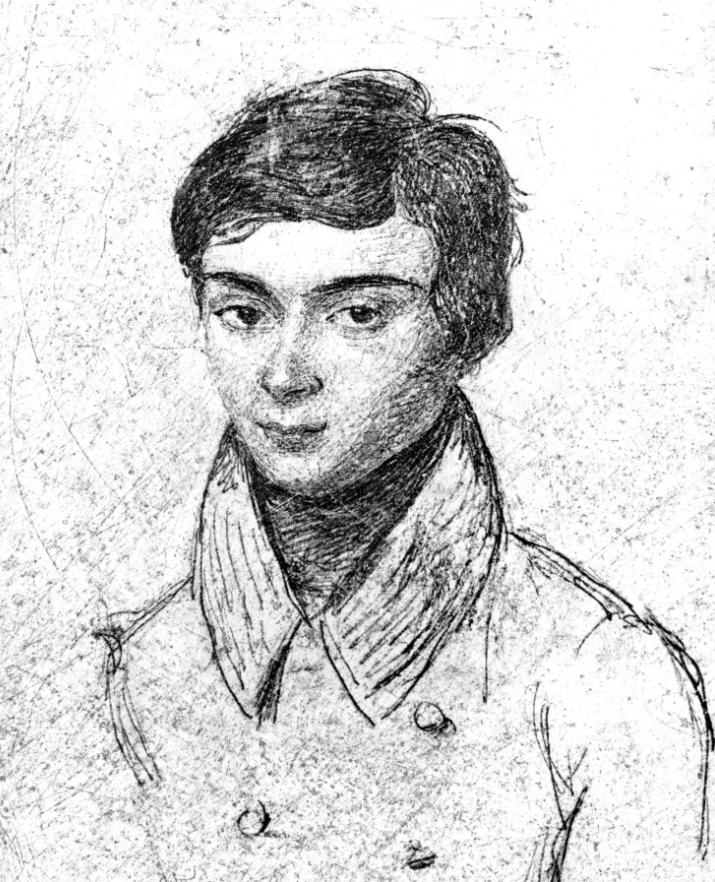
\includegraphics[scale=0.45]{images/galois.png}
\end{center}

Évariste Galois was a French mathematician who lived in the early 1800s. Born on October 25th, 1811 in the village of Bourg-la-Reine, France, Galois’ interest in mathematics started when he was young. He started to seriously study the subject at the age of fourteen when he read the works of contemporary mathematicians such as Legendre; famously precocious, it is said that he understood many of these works completely after the first reading. 

Galois is often credited as being the founder of the modern branch of mathematics known as abstract algebra. This began with him formalizing the definition of a mathematical structure known as a group, which other people had thought of but had never rigorized. From this, Galois laid down some of the fundamental framework of what is now called group theory, which (loosely speaking) is the study of symmetry and the ways in which something can be symmetrical. He also was the first to focus on a field of math aptly named Galois Theory, which is an extension of group theory into other areas of study. Together, these two fields are surprisingly versatile, being used in everything from counting the number of symmetries of a Rubik’s cube to being able to determine whether a given polynomial equation has roots that can be expressed with radicals.

\begin{center}
    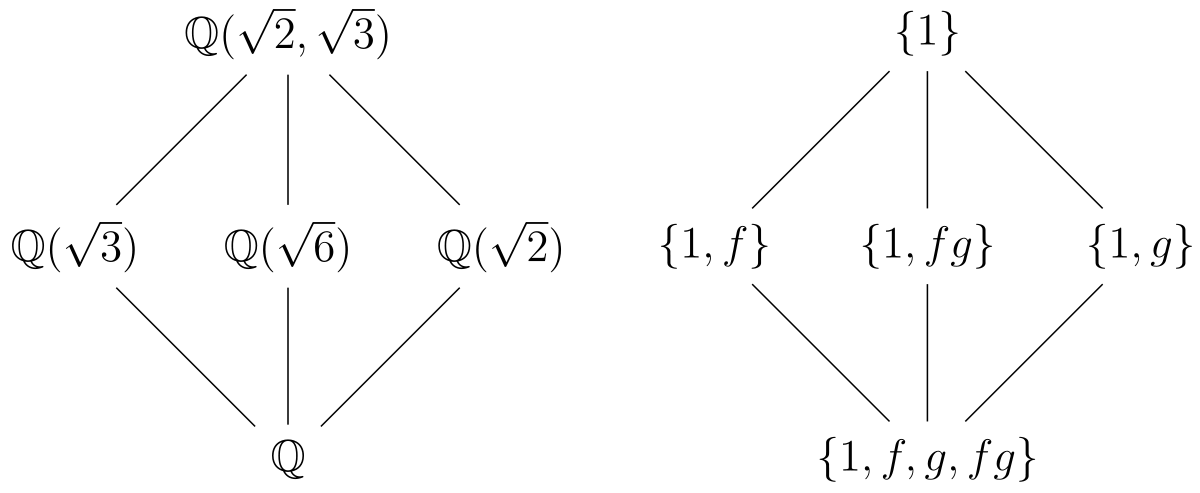
\includegraphics[scale=0.12]{images/galois-theory.png}
\end{center}

Galois might be as well-known for the volatility of his persona as for the genius of his mathematical works. Growing up in a France rocked by political instability, Galois became heavily involved in the Second French Revolution. After making a threatening speech against the king, he was arrested, and then was arrested again shortly after for illegally wearing a uniform. Galois’ time spent in mathematics was also interlaced in this political fervor; at around the same time, Galois was expelled from the French institute École Normale because he attacked the director in a letter to the newspaper. 

Near the end of his life, Galois spent much of his time consolidating all of his mathematical findings into one long letter. Despite it being written very hastily, it touched upon incredibly deep results; some of the theorems he included weren’t proved until more than a century later! 

Shortly after the completion of this letter, Évariste Galois died on May 30th, 1832, in a duel that was likely sparked by political unrest. He was only twenty years old. But despite his unfortunately short life, Galois still is regarded as one of the most important mathematicians of the modern era. Unlike some of his contemporaries, the collection of all his published writing barely spans sixty pages; what they contain, though, is the genesis of some of the fields that are most essential to mathematical research today. And while Galois might ultimately be remembered as perhaps one of the more mysterious figures in math, there is no question that he played an essential role towards getting the subject where it is today.
\end{document}